\documentclass[conference]{IEEEtran}
\IEEEoverridecommandlockouts

\usepackage{cite}
\usepackage{amsmath,amssymb,amsfonts}
\usepackage{algorithm}
\usepackage{algpseudocode}
\usepackage{graphicx}
\usepackage{textcomp}
\usepackage{xcolor}
\usepackage[utf8]{inputenc}
\usepackage[spanish]{babel}
\usepackage{listings}
\usepackage{hyperref}

\def\BibTeX{{\rm B\kern-.05em{\sc i\kern-.025em b}\kern-.08em
    T\kern-.1667em\lower.7ex\hbox{E}\kern-.125emX}}

% Pseudocódigo en español
\algrenewcommand\algorithmicwhile{\textbf{mientras}}
\algrenewcommand\algorithmicdo{\textbf{hacer}}
\algrenewcommand\algorithmicend{\textbf{fin}}
\algrenewcommand\algorithmicif{\textbf{si}}
\algrenewcommand\algorithmicthen{\textbf{entonces}}
\algrenewcommand\algorithmicelse{\textbf{si no}}
\algrenewcommand\algorithmicfor{\textbf{para}}
\algrenewcommand\algorithmicreturn{\textbf{retornar}}
\floatname{algorithm}{Algoritmo}

\begin{document}

\title{Minesweeper en lenguaje ensamblador MARIE.js}

\author{
\IEEEauthorblockN{Alexander Kholodov (00332509), Liam Huang (00335540), Raymond Portilla (00335050)}
\IEEEauthorblockA{CMP-3004.2701: Organización de Computadores\\
Profesor: Felipe Grijalva}
\IEEEauthorblockN{Universidad San Francisco de Quito\\
22 de abril de 2026. Quito, Ecuador}
}

\maketitle

\begin{abstract}
Se implementó el juego Buscaminas sobre el lenguaje ensamblador de MARIE.js. El flujo de trabajo se dividió en dos partes: un script en Python, que genera y visualiza el mapa del juego, y crea un archivo completo \texttt{.mas}; y la lógica base del juego, que gestiona la interacción del usuario, cumplimiento de las reglas del juego, visualización y manejo de celdas en un display $16 \times 16$, y la detección de victoria mediante un contador de celdas restantes.
\end{abstract}

\begin{IEEEkeywords}
MARIE, Assembly, Minesweeper, flood fill, BFS.
\end{IEEEkeywords}

\section{Introducción}

MARIE (\textit{Machine Architecture that is Really Intuitive and Easy}) \cite{null2014essentials} es una arquitectura pedagógica von Neumann con un acumulador de 16 bits, memoria direccionable por palabra de 4096 posiciones y un conjunto de 17 instrucciones. Su simulador web MARIE.js \cite{mariejs} incorpora un display de $16 \times 16$ celdas mapeado direcciones entre \texttt{0xF00} y \texttt{0xFFF}; cada celda admite un valor RGB565 de 16 bits.

Por las limitaciones de la arquitectura ---ausencia de generación aleatoria, interacción a través de la entrada por \texttt{Input} decimal, y control de lazos y condiciones reducido---, la implementación se divide en dos capas: Python prepara los datos (colocación de minas usando la librería \texttt{random}, conteos de vecinos) y MARIE ejecuta la lógica del juego. En estas condiciones surge la necesidad de implementar mucho manualmente, lo que se hace un reto práctico y pedagógico.

\section{Metodología}

\subsection{Enfoque y organización del equipo}

La coordinación del trabajo colaborativo del equipo se fundamentó en el control de versiones en el repositorio de \texttt{GitHub}. Cada miembro del grupo tuvo un rol determinado, que a lo largo del tiempo fue cambiando según los entregables solicitados. El código escrito se basó en talleres, plantillas base del curso y el conjunto de instrucciones oficial de MARIE.js. También, se utilizaron modelos de inteligencia artificial ChatGPT-5.3, ChatGPT-5.3-Codex, Claude Sonnet-4.6, Claude Opus-4.7 en distintas ocaciones, entrenadas con el repositorio \texttt{GitHub}, wiki y conjunto de instrucciones de MARIE.js, y utilizados para asistir en la planificación, escritura y corrección de algunas partes del código. El contenido generado por la inteligencia artificial fue revisado, ajustado, comentado y probado en el simulador manualmente por los autores del proyecto.

\subsection{Generación del tablero en Python}

\texttt{script.py} contiene dos clases. \texttt{MinesweeperBoardGenerator} solicita un número $N$ de minas y los coloca en posiciones únicas con \texttt{random}, y revisa los vecinos para la frontera numérica. El tablero ---matriz $16 \times 16$ con valores en $\{-1, 0, 1, \dots, 8\}$--- se serializa como directivas \texttt{DEC}, precedidas por \texttt{SafeCellsLeft DEC $256-N$} y \texttt{TotalMines DEC $N$}, y se anexa a \texttt{logic.mas} para producir \texttt{marie/buscaminas.mas}. El tablero también se exporta a \texttt{python/board\_data.json}. 

\texttt{MinesweeperVisualizer} lee ese JSON y renderiza el tablero con \texttt{matplotlib}, usando índices 1--16 en ambos ejes. Ejecutar \texttt{script.py} nuevamente sobreescribe los archivos generados sin pasos adicionales.

\begin{figure}[t]
\centering
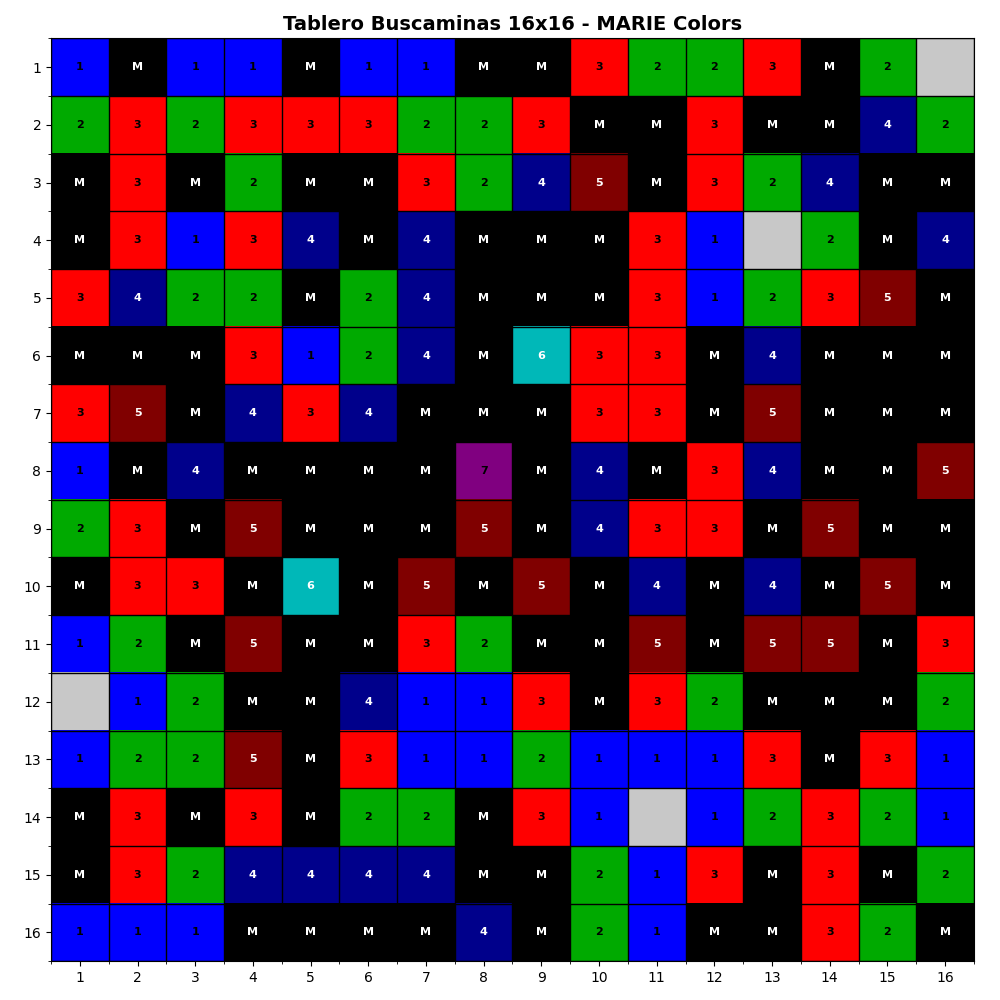
\includegraphics[width=0.85\columnwidth]{figures/Figure_1-script_generated_50.png}
\caption{Generación del tablero por \texttt{script.py} usando \texttt{matplotlib}, con entrada de N=100 minas. Se pueden ver las numeraciones y sus colores RGB565 correspondientes que coinciden con los colores originales de Buscaminas.}
\label{fig:colors}
\end{figure}

\subsection{Lógica de Buscaminas en MARIE.js}

Mientras el mapa es generado por Python debido a la ausencia de \texttt{random} en MARIE.js, la lógica que opera el juego es implementada en el código Assembly del simulador. \texttt{marie/logic.mas} contiene todo excepto el conjunto de posiciones de minas, números y las variables con el número total: se encarga de pedir la entrada del usuario, solicitando las coordenadas con la fila, columna y acción a efectuar sobre la celda buscada, validando el rango de los valores dados. La lógica revisa si la casilla está vacía y en caso de ser así, ejecuta el algoritmo de apertura de celdas vecinas usando Flood Fill BFS, que se detallará a continuación. 

La lógica permite ubicar banderas sobre las casillas con supuestas minas, y en caso de abrir todas las celdas vacías, el juego detecta la victoria del jugador y retorna un mensaje en la sección \texttt{Output log}, anunciando la victoria y mostrando el puntaje obtenido, equivalente al número de minas. Al apuntar a una celda con mina, todas las minas se muestran en el display y se retorna un mensaje anunciando la derrota, revelando el puntaje igual al número de minas que fueron marcadas con bandera exitosamente. A continuación, en las secciones posteriores se explicarán algunos detalles relevantes de la implementación.

\subsection{Mapa de memoria}
El entorno MARIE.js es muy sensible a las direcciones de memoria, que necesariamente deben ser declaradas para ubicar el inicio del arreglo de colores, arreglo de posiciones, etc. Corresponden a las líneas de código del archivo \texttt{marie/buscaminas.mas}, por lo cual se desplazaban al agregar o quitar tan solo una línea de código. El actualizar las categorías de las secciones de memoria fue el proceso más tedioso y frecuente, que se enlistan a continuación:

\begin{itemize}
  \item \texttt{0x100--0x274}: código con la lógica del juego.
  \item \texttt{0x275--0x2C4}: variables, tabla de colores y \textit{Strings} de mensajes.
  \item \texttt{0x2C5--0x3C6}: \texttt{SafeCellsLeft}, \texttt{TotalMines} y las 256 celdas del tablero real.
  \item \texttt{0x400+}: cola del BFS.
  \item \texttt{0xF00--0xFFF}: \textit{framebuffer}, direcciones de memoria de las celdas del display.
\end{itemize}

\subsection{Turnos}

Cada turno consiste en tres llamadas a \texttt{Input} ---fila, columna, acción--- seguidas por sus validaciones (rango 1--16 para coordenadas, 1--2 para acción). \texttt{MoveToCoords} (Algoritmo~\ref{alg:coords}) calcula la dirección absoluta como $DisplayStart + (Row-1) \cdot 16 + (Col-1)$ mediante suma iterativa, que se muestra a continuación:

\begin{algorithm}[H]
\caption{MoveToCoords: coordenadas $\rightarrow$ dirección}
\label{alg:coords}
\begin{algorithmic}[1]
\State $CurrentPos \gets DisplayStart + ColInput - 1$
\State $RowCounter \gets 1$
\While{$RowCounter < RowInput$}
    \State $CurrentPos \gets CurrentPos + 16$
    \State $RowCounter \gets RowCounter + 1$
\EndWhile
\end{algorithmic}
\end{algorithm}

\subsection{Algoritmo de revelado de celdas vacías usando Flood Fill BFS}

Revelar una celda numérica ($1$--$8$) pinta el color correspondiente y decrementa \texttt{SafeCellsLeft}. Revelar una celda con valor $0$ dispara una propagación BFS (Algoritmo~\ref{alg:flood}) con cola en \texttt{0x400} y punteros \texttt{QueueHead}, \texttt{QueueTail}. Para cada celda desencolada se evalúan las ocho direcciones, verificando antes de cada una su frontera: \texttt{ColCalc} (índice de columna $0$--$15$, obtenido por restas sucesivas de 16 en \texttt{ColMod}) se compara contra $0$ con \texttt{Skipcond 800} (borde izquierdo) y contra $15$ con \texttt{Subt Fifteen}$+$\texttt{Skipcond 000} (borde derecho); \texttt{ProcOffset} (desplazamiento lineal $0$--$255$ desde \texttt{DisplayStart}) se compara contra $16$ con \texttt{Subt DisplayWidth}$+$\texttt{Skipcond 000} (borde superior) y contra $240$ con \texttt{Subt TwoForty}$+$\texttt{Skipcond 000} (borde inferior). Las ocho direcciones comparten \texttt{CheckReveal}: aplica el filtro (oculta y no mina), pinta, decrementa \texttt{SafeCellsLeft}, evalúa victoria y encola sólo si el valor de la celda es $0$.

\begin{algorithm}[H]
\caption{Flood Fill iterativo (BFS)}
\label{alg:flood}
\begin{algorithmic}[1]
\State encolar celda inicial
\While{cola no vacía}
    \State $c \gets$ desencolar
    \For{cada vecino $v$ de $c$ dentro del tablero}
        \If{$v$ oculta \textbf{y} $v$ no es mina}
            \State pintar $v$ con su color
            \State $SafeCellsLeft \gets SafeCellsLeft - 1$
            \If{$SafeCellsLeft = 0$} \State ir a victoria \EndIf
            \If{valor de $v == 0$} \State encolar $v$ \EndIf
        \EndIf
    \EndFor
\EndWhile
\end{algorithmic}
\end{algorithm}

\subsection{Banderas y puntaje}

\texttt{ToggleFlag} alterna entre oculto y bandera sobre celdas no reveladas. Marcar una mina incrementa \texttt{Score}; desmarcarla lo decrementa. El valor de \texttt{Score} no se muestra durante la partida, se retorna en \texttt{Output log} al finalizar el juego. La mecánica de banderas considera el caso especial de tratar de revelar la celda marcada: mientras una celda está marcada con bandera, no se puede revelar sin desmarcarla previamente. La consideración este y otros casos especiales en las mecánicas demuestra la robustez y completitud de la implementación del juego dentro del presente proyecto.

\subsection{Fin del juego y salida}

La victoria ocurre cuando \texttt{SafeCellsLeft} llega a cero. El contador, inicializado a $256-N$ por Python, se decrementa en cada revelado (directo o propagado). Si el contador de celdas vacías llega a cero, se declara la victoria y el \texttt{Score} muestra en \texttt{Output log} el puntaje máximo alcanzable, equivalente a \texttt{TotalMines}.

La derrota ocurre al revelar una mina. \texttt{GameOver} pinta la celda pulsada de negro y recorre todo el tablero pintando de negro las minas restantes. \texttt{Score} conserva el valor acumulado, reflejando cuántas minas el jugador había marcado con bandera correctamente hasta el momento de perder.

En ambos casos el programa emite un mensaje: \texttt{PrintMsg} recorre la memoria desde \texttt{MsgPtr} llamando a \texttt{Output} por cada símbolo hasta encontrar un nulo. Ambos \texttt{MsgDefeat} y \texttt{MsgWin} son \texttt{Strings} ASCII en \texttt{DEC}. 

\subsection{Impresión del puntaje a ASCII}

La función \texttt{PrintScore} convierte \texttt{Score} ($0$--$256$) a tres dígitos decimales mediante restas iteradas: resta 100 repetidamente contando las veces hasta que el acumulador se vuelve negativo (centenas), luego repite con 10 (decenas), y el residuo es las unidades. Cada dígito se emite sumándole \texttt{AsciiZero} ($48$) para producir el código ASCII correspondiente, haciendo tres llamadas consecutivas a \texttt{Output}.

\section{Resultados}

El sistema mostró ser funcional y robusto en su implementación, minimizando el efecto de interacción no deseada de parte del usuario, a través de validaciones y casos especiales. A continuación se mostrará un ejemplo de ejecución del programa \texttt{buscaminas.mas} en MARIE.js.

En la Fig.~\ref{fig:initial} se puede observar el estado del tablejo inicial, con todas las casillas ocultas. Al ingresar 1-3-1 (abrir la casilla en las coordenadas (1;3)), se reveló toda la región vacía adyacente a esta celda hasta las fronteras numéricas de las minas, lo que se puede visualizar en la Fig.~\ref{fig:flood}. Esta implementación mostró ser eficiente y el tiempo necesario para ejecutar el algoritmo es muy bajo.

\begin{figure}[t]
\centering

\includegraphics[width=0.65\columnwidth]{figures/Figure_2-empty.png}
\caption{Estado inicial del tablero en el display de MARIE.js: 256 celdas ocultas (gris oscuro).}
\label{fig:initial}
\end{figure}

\begin{figure}[t]
\centering
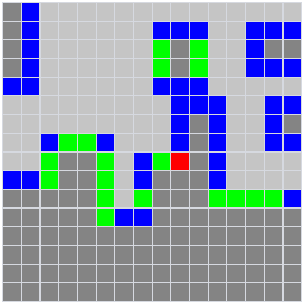
\includegraphics[width=0.65\columnwidth]{figures/Figure_3-flood_reveal.png}
\caption{Resultado de la apertura de una región de celdas vacías usando Flood Fill BFS. Nota: el mapa tiene más celdas vacías, pero no son adyacentes a la región revelada, por lo cual permanecen ocultas.}
\label{fig:flood}
\end{figure}

Se han ejecutado varios comandos, ubicando tres banderas en las posiciones (1;1), (4;1) y (3;15), donde se esperan las minas. Se verificaron casos límite: no se puede revelar una celda con bandera; colocar bandera sobre una celda ya revelada o frontera numérica no produce efecto. Al tratar de abrir la celda (16;1), explosiona una mina y se revelan todas las bombas en el mapa, como se puede ver en la Fig.~\ref{fig:defeat}. El mensaje del anuncio de la derrota se muestra en la consola, seguido puntaje acumulado hasta el momento (3).

\begin{figure}[t]
\centering
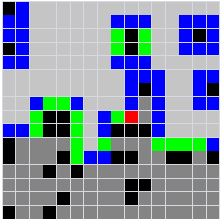
\includegraphics[width=0.65\columnwidth]{figures/Figure_5-defeat_parcial_score.png}
\caption{Apertura de una mina que resulta en revelación de todas las minas en el tablero (incluyendo las casillas que fueron marcadas con bandera; en esta jugada, tres fueron marcadas). \texttt{Output log} retorna el mensaje: ``\textit{Defeat! Score: 003}'', que corresponde a las tres minas marcadas correctamente antes de la derrota.}
\label{fig:defeat}
\end{figure}


\section{Conclusiones}

Se concluye que el sistema mostró ser funcional, robusto, balanceando la eficiencia y la longitud del código, considerando los casos límite de la interacción del usuario. El proyecto y todos sus entregables cumplen con las instrucciones dadas en clase y enlistadas en la página de \texttt{Notion}.

El trabajo en equipo durante este proyecto resultó ser cómodo y eficiente mediante la separación de roles y control de versiones en \texttt{GitHub}. Los mayores retos fueron la implementación de flood fill con BFS iterativo y cola en memoria, el recorrido de celdas con punteros, la actualización constante de direcciones de memoria, y la gestión de multiplicación y división en las funciones.

\begin{thebibliography}{00}
\bibitem{null2014essentials} L. Null and J. Lobur, \textit{The Essentials of Computer Organization and Architecture}, 5th ed. Burlington, MA: Jones \& Bartlett Learning, 2018.
\bibitem{mariejs} MARIE.js contributors, GitHub. \url{https://github.com/MARIE-js/MARIE.js}, 2026. MIT License.
\end{thebibliography}

\end{document}